\documentclass{beamer}
\usetheme{Boadilla}
\usepackage{mathtools}
\usepackage{amssymb,array}
\usepackage{graphicx}
\usepackage[square]{natbib} 

\usepackage[utf8]{inputenc}
 
 
%Information to be included in the title page:
\title{Relaxed Radix Balanced Trees}
\author{Elias Khoury}
\date{2016}
 
 
 
\begin{document}
 
\frame{\titlepage}
 
\begin{frame}
\frametitle{Background}

\begin{itemize}

	\item Invented by researchers at EPFL in Lausanne\cite{bagwell2011rrb} \pause
	\item RRB-Trees are part of the ongoing development of the Scala Programming Language \pause
	\item The goal is to present a datastructure which can be concatenated in O(log n) time at no cost to other operations \pause

\end{itemize}

\end{frame}
 
\begin{frame}

\frametitle{Application}

\begin{itemize}

	\item RRB-Trees can be used to implement an efficient vector datastructure
	\item As it is a purely functional datastructure the operations on it can be easily run in parallel  
	\item An application for efficient vector concatenation is:

\end{itemize}

\end{frame}
 
\begin{frame}
\frametitle{Main Concept}


\begin{itemize}

	\item To represent a vector as a tree structure \pause
	\item Multiple variables to control:
		\begin{itemize}
			\item Branching factor
			\item Balance of the tree
		\end{itemize}
	\pause
	\item The main operations are:
	\noindent\parbox[t]{2.4in}{\raggedright%
		\begin{itemize}
			\item Indexing
			\item Updating
		\end{itemize}
	}%
	\noindent\parbox[t]{2.4in}{\raggedright%
		\begin{itemize}
			\item Append to the front or back
			\item Splitting
		\end{itemize}
	}%

\end{itemize}

\end{frame}

\begin{frame}
\frametitle{The Problem}

Given two trees of branching factor m, a naive approach will simply be a copy of linear cost from one tree to another. Likewise a naive O(1) solution is possible, but at the cost of degenerating the datastructure into a linked list

	\begin{center}
	
	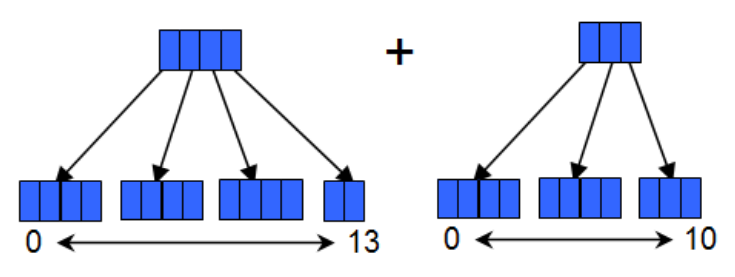
\includegraphics[scale=0.3]{joinvectors.png}
	
	\end{center}

\end{frame}


\begin{frame}
\frametitle{Radix Search}

	\begin{itemize}
	
		\item With a perfectly balanced tree of branching factor m, for any particular sub branch, there are exactly $m^{h-1}$  leaves. Therefore, an index i can be found using $\lfloor i / (m^{h-1}) \rfloor$ 
	\end{itemize}
	\begin{center}
	
	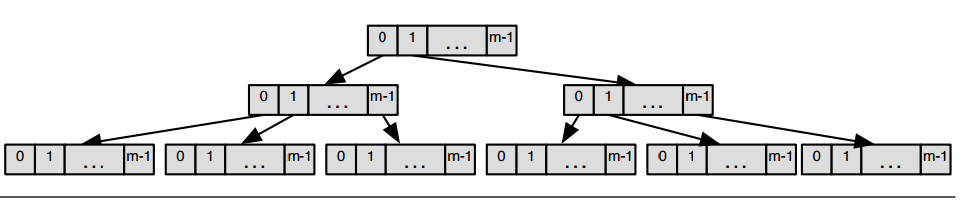
\includegraphics[scale=0.25]{radixbalancedtree.png}
	
	\end{center}
	
	eg. For m = 4. Finding the index 5 using the tree above yields the following calculations:
	\begin{tabular}{l l}
	
	$\lfloor 5 / (4^{3-1}) \rfloor = 0$ & $ \lfloor 5 / (4^{1-1}) \rfloor = 5 $ \\
	$\lfloor 5 / (4^{2-1}) \rfloor = 1$ & $ 5 \quad \% \quad 4 = 1 $ \\
	
	\end{tabular}		

\end{frame}


\begin{frame}
\frametitle{Relaxed Radix Search}

	\begin{itemize}
		\item However, for this particular application we need to relax the branching factor m in order to circumvent the linear concatenation cost.
		\item The concept of a variable branching factor has been applied to tree structures before, like 2-3 Trees and finger trees
		\item By relaxing the branching factor, we lose the guarantee that any leaf node can be found in O(1) time, this is due to the possibility of the tree being slightly unbalanced. 
		\item The cost this adds is a slight linear lookup when arriving at a node that is unbalanced.
	
	\end{itemize}

\end{frame}

\begin{frame}
\frametitle{Branching Factor and Balance}

	\begin{itemize}
		\item Having a variable branching factor makes it more difficult to maintain a balanced structure. \pause
		\item A good way of still being able to maintain the convenience of a balanced tree is to simply state the size of each unbalanced subtree. \pause
		\item Furthermore, choosing the upper and lower bounds of the branching factor can help determine how unbalanced the tree could become. \pause
		\item For a tree of branching factor m, the height h is $log_m (n)$. Therefore, given two possible values of m. the ratio of the heights is $\frac{log_{m_{min}}}{log_{m_{max}}}$ \pause
		\item The closer to 1 this ratio is the more balanced the tree is. Choosing $m_{max} = m_{min} + 1$ is a good compromise. \pause
	
	\end{itemize}
	
	\begin{center}
	
	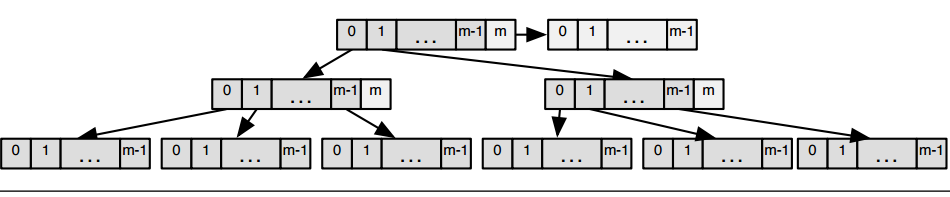
\includegraphics[scale=0.25]{relaxedradixbalancedtree.png}
	
	\end{center}

\end{frame}
 
 
\begin{frame}
\frametitle{RRB-Trees}

	\begin{itemize}
	
		\item The concatenation operation works by effectively merging the right side of the left tree, with the left side of the right tree. 
		\item starting from the leaf nodes of both trees, a new tree is built from the bottom up containing the merged data of both trees.
		\item The concept behind this is to use the concept of sharing when building this new tree in order to minimise the cost of copying data
		\item For a tree of height, h. The complexity of this operation is O(Log(h)). However, there is a significant constant time cost when it comes to ensuring that the merged tree is balanced
	
	\end{itemize}

\end{frame}
 
 
\begin{frame}
\frametitle{Concatenation Process}

	\begin{center}
	
	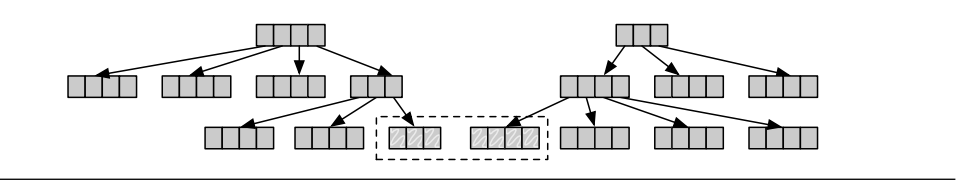
\includegraphics[scale=0.3]{concat1.png}
	
	\end{center}
	
	merge the leaf nodes of each tree to create a new tree of height 1

\end{frame}

\begin{frame}
\frametitle{Concatenation Process}

	\begin{center}
	
	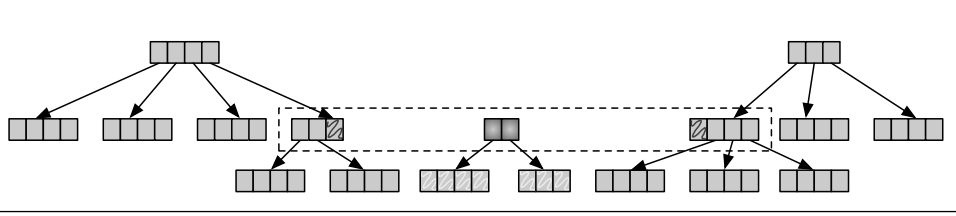
\includegraphics[scale=0.3]{concat2.png}
	
	\end{center}
	
	propagate the merge up the tree. Note: At each stage of the merge the tree needs to be rebalanced

\end{frame}

\begin{frame}
\frametitle{Concatenation Process}

	\begin{center}
	
	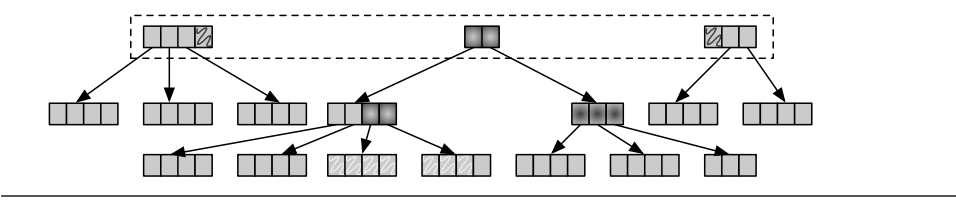
\includegraphics[scale=0.3]{concat3.png}
	
	\end{center}
	
	Only the highlighted nodes need to be modified. The rest are simply shared.	
	
	\begin{center}
	
	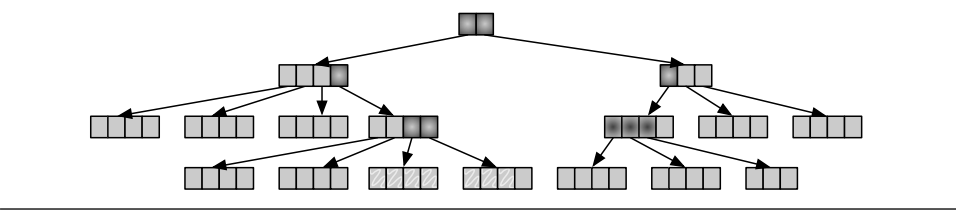
\includegraphics[scale=0.3]{concat4.png}
	
	\end{center}
\end{frame}

\begin{frame}
\frametitle{A note on branching factor}

	\begin{itemize}
		\item For simplicity of the diagrams a branching factor of 4 was chosen
		\item In practice the most efficient branching factor is actually 32
		\item Branching factor controls tree height which affects the runtime of the operations
		\item Need to minimise branching factor without degenerating into a linked list
	\end{itemize}
	
	\begin{center}
	\begin{tabular}{| l || c | c |}
		\hline
		& RRB-Vector & With m = 32 \\
		\hline
		indexing & $ log_m $ & eC\\
		update & aC & eC \\
		insert ends & $ m \times log_m $ & aC \\
		concat & $ m^2 \times log_m $ & L v.s. eC \\
		split & $ m \times log_m $ & eC \\
		\hline
		\end{tabular}
	\end{center}


\end{frame}

\begin{frame}
\frametitle{Runtime Complexity In Relation To Similar Structures}

	\begin{center}
	\begin{tabular}{| l || c | c | c |}
		\hline
		& RRB-Vector & Finger Tree & Red-Black Tree\\
		\hline
		indexing & eC & $ Log_2 $ & $ Log_2 $ \\
		update & eC & $ Log_2 $ & $ Log_2 $\\
		insert ends & aC & aC & $ Log_2 $\\
		concat & L v.s. eC & $ Log_2 $ & L\\
		split & eC & $ Log_2 $ & $ Log_2 $\\
		\hline
		\end{tabular}
	\end{center}

\end{frame}

\begin{frame}

\bibliographystyle{abbrvnat}
\bibliography{/home/elias/Documents/G52AAD/RRB-Trees/data/Presentation}

\end{frame}

\end{document}